\documentclass[sigplan,screen]{../acmart}

\AtBeginDocument{%
  \providecommand\BibTeX{{Bib\TeX}}%
}

\setcopyright{none}
\settopmatter{printacmref=false, printccs=false}
\copyrightyear{2026}
\acmYear{2026}
\acmDOI{}
\acmConference[Draft]{Draft manuscript}{June 2026}{Busan, Republic of Korea}
\acmISBN{}

\usepackage{kotex}
\usepackage{booktabs}
\usepackage{bbm}
\usepackage{siunitx}
\graphicspath{{../}{../figures/}}
\newcommand{\Ind}{\mathbbm{1}}
\providecommand{\correspondingauthor}{}

\title{PUBG 텔레메트리의 시공간 데이터베이스 모델링과 페이즈 단위 팀 탈락 예측}

\author{Seong Eun BAEK}
\email{todtjddms104204@pusan.ac.kr}
\correspondingauthor
\authornotemark[1]
\affiliation{%
  \institution{Pusan National University}
  \city{Busan}
  \country{Republic of Korea}
}

\author{Joonho KWON}
\email{jhkwon@pusan.ac.kr}
\affiliation{%
  \institution{Pusan National University}
  \city{Busan}
  \country{Republic of Korea}
}

\begin{abstract}
배틀로얄 생존은 경기 종료 후의 단일 순위가 아니라 안전 구역 수축에
따라 변하는 위험 과정이다. 본 연구는 공식 PUBG 텔레메트리를 이동하는
팀, 동적 안전/블루존, 공간 이벤트, 팀 관계를 포함하는 시공간
데이터베이스(STDB)로 재구성하고, 재구성한 존 변화 구간에 인덱스를
부여해 팀 단위 다음 페이즈 탈락 위험 예측 문제를 정의한다. 그래프 구성이 가능한
21,824개 경기에서 66차원 팀-페이즈 특징과 근접, 교전, 공동 안전존
압력을 나타내는 3채널 동적 그래프를 구축하였다. 특징만 사용하는
gradient boosting 모델도 AUC 0.765로 강한 성능을 보였지만, 동적
그래프를 사용하는 DynamicSTGNN은 134,245개 정렬 테스트 셀에서
AUC 0.778, AP 0.681까지 향상되었다. 표현 ablation은 텔레메트리
기반 표현이 전략 점수 요약의 AUC 0.649를 0.765까지 끌어올린다는 점을
보였고, 그래프 ablation과 shuffle control은 동적 팀
관계가 특징만으로는 설명되지 않는 작지만 유의한 신호를 제공함을
보였다. 결과적으로 가장 큰 이득은 페이즈 정렬 텔레메트리 표현에서
나오며, 동적 그래프는 그 위에 관계 신호를 추가한다.
\end{abstract}


\keywords{PUBG 텔레메트리, 시공간 데이터베이스, 동적 그래프, 생존 모델링, 게임 분석}

\begin{document}

\maketitle

\section{서론}

배틀로얄 경기의 최종 순위는 플레이 가능 영역이 축소되면서 변하는
생존 위험이 누적된 결과이다. \textit{PUBG: Battlegrounds}에서
플레이어는 낙하하고, 아이템을 획득하고, 교전하며, 점점 줄어드는
전장에서 마지막까지 생존해야 한다. 블루존 바깥에 오래 머무르면
체력이 감소하므로 플레이어는 계속 이동 압력을 받는다
~\cite{pubgGameInfo}. 경기 중 안전 구역 갱신과 블루존 이동은
텔레메트리에서 관측 가능한 존 변화 구간을 형성한다. 본 연구는
각 구간에 인덱스를 부여하여 \textit{분석 페이즈}로 사용함으로써, 공간 수축
과정의 비교 가능한 시점에서 생존 위험을 측정한다. 이 표현에서는 같은
피해량, 이동 거리, 적과의 조우도 현재의 존 압력과 안전 구역 기하에
따라 다른 위험을 의미한다. 따라서 경기 종료 후 집계 통계만으로는 팀이
언제 취약해졌고 어떤 공간 조건이 그 위험을 만들었는지 설명하기 어렵다.

본 연구는 공식 PUBG 텔레메트리를 팀 관점에서 분석한다. 개발자 API는
시간에 따른 플레이어 위치, 교전, 존 상태 변화 이벤트, 탈락을
기록한다~\cite{pubgDeveloperPortal,pubgTelemetryEvents,pubgTelemetryObjects}.
우리는 플레이어 기록을 팀 궤적, 존 노출, 팀 간 관계로 집계하고,
마지막 생존 팀원이 탈락한 시점을 팀 탈락 시점으로 정의한다. 핵심 예측
문제는 인덱싱된 분석 구간 \(k\) 종료 시점까지 관측 가능한 정보만으로
해당 팀이 다음 구간 \(k+1\) 동안 탈락하는지를 예측하는 것이다. 이를
이산시간 event-history 관점의 \textit{다음 페이즈 탈락 위험}으로 정의한다
~\cite{allison1982discrete,singer1993discrete}.

본 논문은 두 질문을 다룬다. \textbf{RQ1}: 공식 PUBG 텔레메트리를
페이즈 정렬 STDB로 재구성하여 팀 궤적, 존 노출, 교전 이벤트, 동적
팀 관계를 특징과 그래프로 도출할 수 있는가? \textbf{RQ2}: 이 표현
위에서 특징 기반 모델은 다음 페이즈 탈락 위험을 얼마나 잘 예측하며,
동적 그래프는 특징만으로 설명되지 않는 추가 신호를 제공하는가?
기여는 세 가지이다. 첫째, 팀 단위 페이즈 수준 생존 위험 예측 문제를
정의한다. 둘째, 21,824개 경기의 페이즈 정렬 STDB 표현을 구축한다.
셋째, 표현 자체의 이득과 그래프 관계의 추가 이득을 실험적으로
분리한다.

\section{배경}
\label{sec:background}

대부분의 PUBG 예측 연구는 경기 종료 후 통계를 이용해 최종 순위를
예측한다~\cite{kagglePubgFinishPlacement,sen2021pubgFinalRank,lee2025pubgRank}.
이 접근은 최종 결과 모델링에는 적합하지만, 위험이 발생한 시간적
순서와 공간 맥락을 제거한다. 가장 가까운 선행 연구는 Sagong 등의
페이즈 기반 프레임워크이다. 이 연구는 FightScore와 ActiveScore로
플레이어의 공격성과 활동성을 점수화하고, 전략 유형을 군집화한 뒤
다음 페이즈 생존을 예측한다~\cite{sagong2025hunterCamper}. 우리는
페이즈 수준 문제 설정을 계승하되, 분석 단위를 플레이어에서 팀으로
바꾸고 작은 전략 점수 요약 대신 전체 텔레메트리 재구성을 사용한다.

수축하는 안전 구역은 시공간적 관점도 요구한다. 서식지 단편화와
movement ecology는 이용 가능한 공간, 이동, 노출, 밀도를 서로 결합된
시간-공간 변수로 다룬다
~\cite{fahrig2003fragmentation,nathan2008movement}. 우리는 이를
생물학적 주장으로 사용하지 않고 분석적 비유로만 사용한다. PUBG 팀은
유기체가 아니지만, 그들의 생존 조건은 축소되는 활동 공간에 의해
형성된다. 따라서 각 페이즈를 특징 행과 그래프 스냅샷으로 동시에
표현한다. 그래프 edge는 어느 팀이 가까운지, 어느 팀이 누구를
공격했는지, 어떤 팀들이 같은 안전존 압력을 받는지를 인코딩한다
~\cite{sanchezLengeling2021gnnIntro}.

\section{방법}
\label{sec:methods}

공식 텔레메트리를 수집하고, 공통 시간축과 지도 좌표축 위에서 네
종류의 STDB 객체로 재구성한다. 네 객체는 이동하는 팀, 동적
안전/블루존, 공간 이벤트, 페이즈 구간이다. 튜토리얼/훈련장 경기와
소수의 비정상 텔레메트리를 제외한 뒤, 그래프 구성이 가능한 경쟁
경기 21,824개를 사용하였다. 재구성한 존 변화 구간을 분석 페이즈
1--8로 인덱싱하고, 예측 기준 페이즈는 1--7로 둔다.
구현상 STDB는 팀 상태, 존, 이벤트, 팀-페이즈, 간선 릴레이션으로
구체화된다. 팀 상태는 경기, 팀, 페이즈, 시간, 좌표, 생존 여부를 담고,
존은 중심, 반경, 시작/종료 시점을 담으며, 이벤트는 위치와 공격/피해 팀 및
이벤트 유형을 기록한다. 팀-페이즈와 간선 릴레이션은 각각 특징/목표값과
출발 팀, 도착 팀, 관계 유형, 가중치를 담아 모델 입력 행과 그래프로 변환된다.

\begin{figure}[htbp]
\centering
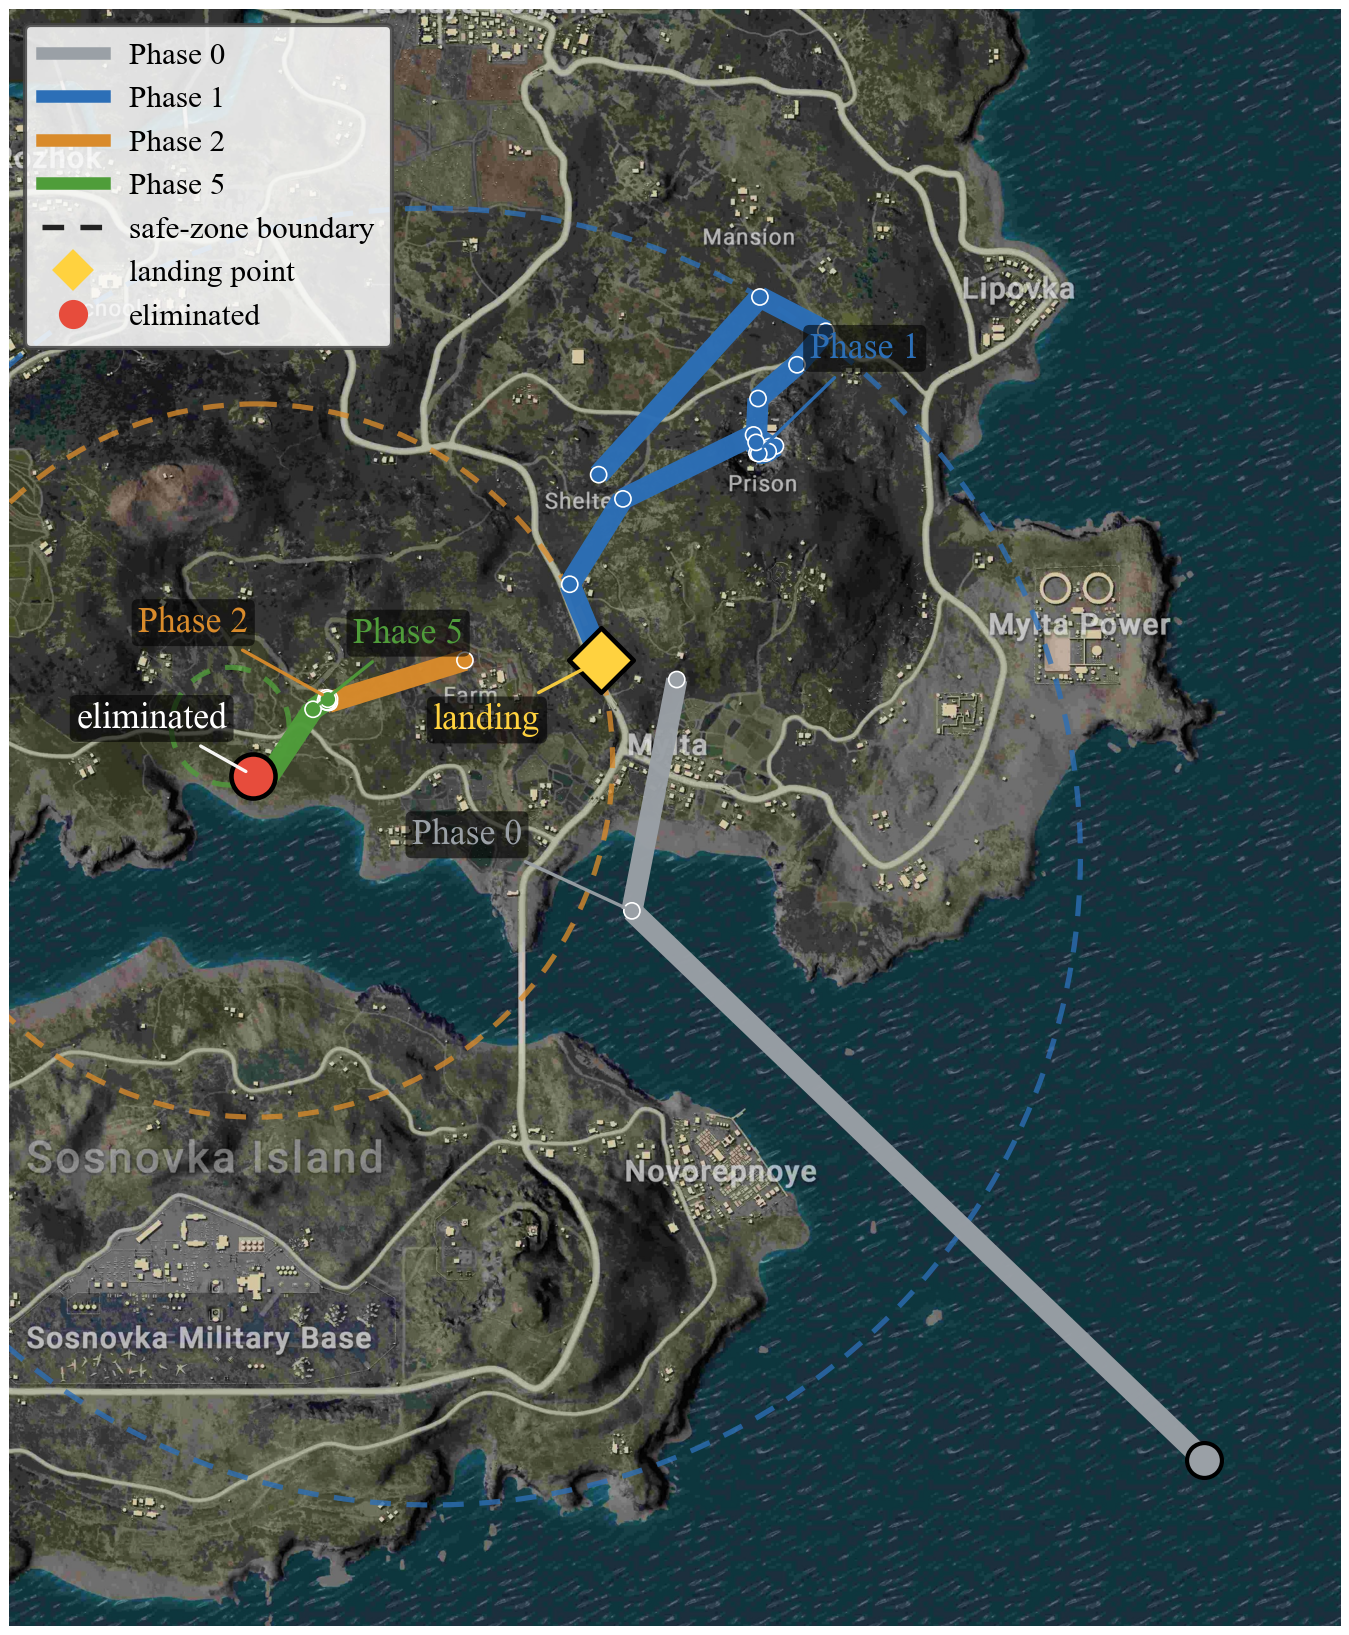
\includegraphics[width=0.88\linewidth]{figures/team_phase_feature_example.png}
\caption{팀-페이즈 STDB 예시. 팀 centroid 궤적을 페이즈별 안전 구역
경계와 정렬하고, landing point, phase movement, elimination point를
하나의 페이즈 인덱스 공간 이력으로 표현한다.}
\label{fig:team-phase-feature-example}
\end{figure}

\paragraph{팀-페이즈 특징.}
모델링 단위는 \((m,i,k)\), 즉 경기 \(m\), 팀 \(i\), 페이즈 \(k\)이다.
각 행은 한 팀의 페이즈 내 이동 궤적, 존 노출, 교전, 상태, 준비도를
요약한다. 표~\ref{tab:feature-sources}에서는 모델 입력의 원천을 기존
텔레메트리 집계와 STDB 시공간 표현으로 나눈다.
\(d\)는 표현 ablation에서 HGB가 사용한 tabular 입력 수이다.
DynamicSTGNN은 같은 원천에서 중복 페이즈 항목과 비수치 표현을 정리한
66개 정규화 수치 노드 특징을 사용한다. 따라서 표의 결합 표현
\(d=72\)와 DynamicSTGNN의 \(F=66\)은 같은 원천을 서로 다른 입력 관점으로
정리한 값이다. STDB 시공간 단독 표현의 16개 변수 중 \(phase\_idx\)는
기존 집계에도 포함되는 공통 cut index이므로, 결합 표현에서는 신규 STDB
변수 15개만 추가된다.

\begin{table}[htbp]
\centering
\caption{기존 텔레메트리 집계와 STDB 시공간 표현의 구분.}
\label{tab:feature-sources}
\scriptsize
\setlength{\tabcolsep}{2.5pt}
\begin{tabular}{p{0.18\linewidth}p{0.22\linewidth}rp{0.42\linewidth}}
\toprule
구분 & 특징군 & \(d\) & 대표 특징 \\
\midrule
기존 집계 & 경기/팀 상태, 교전, 준비도 & 57 &
페이즈 길이, 생존 팀/플레이어 수, 체력, 차량, 팀 분산, 피해량, 기절,
처치, 교전 상대, 아이템, 회복/부스트 \\
STDB 시공간 단독 & 궤적, 존/적 노출 & 16 &
페이즈 인덱스, 팀 centroid 이동 거리, 순변위, 속도, 회전 시점, 안전 구역 방향 정렬,
진입 시점, 경계 거리, 블루존 밖 체류 비율, 주변 적 밀도, 최근접 적 거리 \\
결합 표현 & 기존+STDB 시공간 & 72 &
기존 집계와 STDB 궤적/노출 특징을 결합하되, 공통 페이즈 인덱스를 한 번만
센 탈락 위험 예측 입력 \\
\bottomrule
\end{tabular}
\end{table}

팀 위치는 생존 팀원의 centroid로 계산하고, 팀 분산과 최근접 적 관련
변수는 분산된 squad 상황을 보완한다. 모든 특징은 해당 페이즈 내부
관측치에서만 계산하며, 특징별 고정 상수로 스케일링한다. 피해량, 아이템
획득, 교전 이벤트 횟수처럼 드물게 큰 값이 나타나는 변수는 로그 압축한다.
DynamicSTGNN의 각 팀-페이즈 노드는 이 원천들을 정규화한 66차원 벡터로
표현된다.
그림~\ref{fig:team-phase-feature-example}에서는 이 행 단위 표현이 포착하는
공간적 관점을 보여준다.

\paragraph{동적 팀 그래프.}
각 페이즈에 대해 가중 heterogeneous graph
\(G_k=(V_k,X_k,\{A_k^r\}_{r\in R})\)를 정의한다. 노드는 팀이고,
\(X_k\)는 특징 행렬이며, \(R\)은 세 관계 채널을 포함한다. 근접
관계는 팀 centroid 사이의 거리 감쇠 대칭 간선이다. 교전 관계는
공격자에서 피해자로 향하는 방향 간선이며, 피해량, 기절, 처치에
따라 가중치가 증가한다. 공동 압력 관계는 함께 안전 구역 밖에 있거나
안전 구역 경계 근처에 있는 인접 팀을 연결한다. 모든 관계 채널은
페이즈 \(k\) 내부 관측치만으로 계산한다. 그래프 집계 전에는 각 팀에서
나가는 관계 가중치의 합이 1이 되도록 조정하여, 연결된 상대 팀들의
정보를 링크 수 자체에 좌우되지 않게 결합한다. 근접 관계에서는 팀
자신의 특징도 함께 유지한다. 그림~\ref{fig:dynamic-graph-example}에서는
페이즈 수준 STDB snapshot이 모델 입력 그래프 구조로 변환되는 과정을
보여준다.

\begin{figure*}[htbp]
\centering
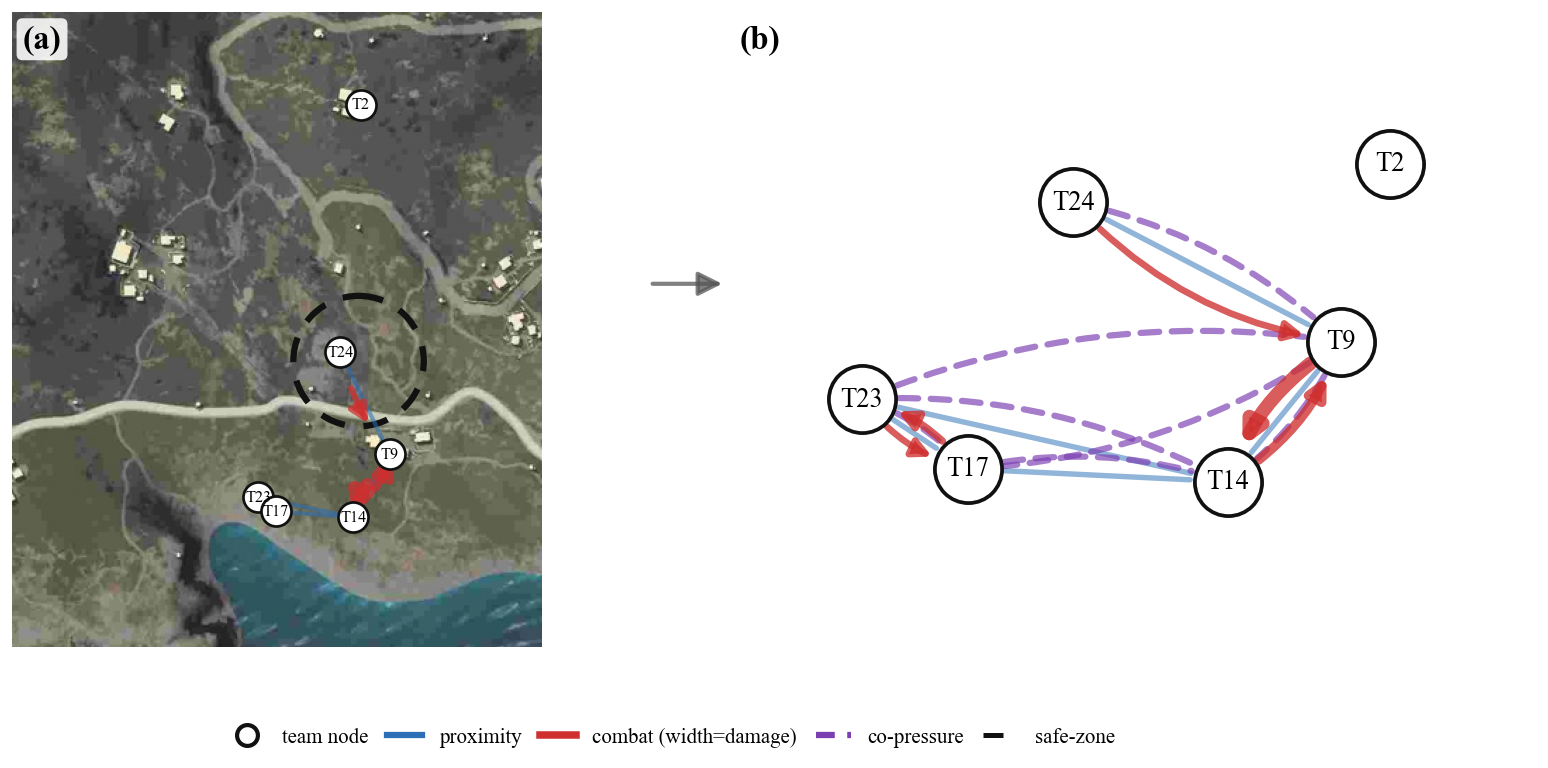
\includegraphics[width=0.78\textwidth]{figures/dynamic_heterogeneous_graph_example.png}
\caption{동적 heterogeneous graph 예시. 팀 centroid, 안전 구역 경계,
교전 이벤트를 포함한 phase-level STDB snapshot을 팀 사이의 근접, 교전,
공동 압력 관계로 변환한다.}
\label{fig:dynamic-graph-example}
\end{figure*}

\paragraph{위험 예측 문제와 모델.}
각 분석 페이즈의 종료 시점에서 아직 생존해 있고 다음 구간이 관측되는
팀만 위험 집합에 포함한다. \(b_k\)를 페이즈 \(k\)의 종료 시점,
\(T_i\)를 팀 \(i\)의 탈락 시점이라 하자. 이진 목표 변수는 다음과 같다.
\[
Y_{i,k}=\Ind\!\left\{b_k < T_i \leq b_{k+1}\right\}, \qquad
h_{i,k}=P(Y_{i,k}=1 \mid T_i>b_k, X_{i,\leq k}).
\]
즉 \(Y_{i,k}=1\)은 팀 \(i\)가 \(b_k\)까지 생존했지만 다음 페이즈가 끝나기
전에 탈락했음을 의미한다. \(b_k\) 시점에 이미 탈락한 팀, 패딩된 팀 슬롯,
다음 페이즈가 관측되지 않는 셀은 분석과 손실 계산에서 제외한다.

DynamicSTGNN은 팀-페이즈 특징의 시간 순서와 근접, 교전, 공동 압력 그래프의
시간 순서를 함께 입력으로 받는다. 모델은 각 팀의 시간적 변화와 팀 사이의
관계를 함께 요약한 뒤, 각 기준 페이즈마다 다음 구간 탈락 위험 점수를 출력한다.
구체적으로 \(X\in\mathbb{R}^{B\times T\times N\times F}\)와
\(A\in\mathbb{R}^{B\times T\times E\times N\times N}\)를 입력으로 받으며,
\(T=8\), \(N_{\max}=128\), \(F=66\), \(E=3\)이다. 입력층은 노드 특징을
64차원 상태로 사상하고, 두 개의 spatio-temporal block을 통과시킨다. 각
block은 gated causal temporal convolution, 관계별 graph aggregation, 두 번째
causal temporal convolution, layer normalization과 residual connection으로
구성된다. Temporal convolution은 phase \(k\)가 \(k\) 이후 정보를 보지 못하게
하고, 패딩 팀과 위험 집합에 속하지 않는 셀은 graph 집계와 손실 계산에서
mask한다.

\section{실험 및 결과}
\label{sec:results}

\paragraph{평가 프로토콜.}
하나의 경기는 여러 팀과 여러 분석 페이즈를 만들기 때문에, 팀-페이즈
행을 무작위로 나누면 같은 경기의 공간 조건과 교전 맥락이 훈련과 테스트에
동시에 들어갈 수 있다. 이를 피하기 위해 seed 42에서 경기 단위로
17,460개 훈련, 2,182개 검증, 2,182개 테스트 경기를 분할하였다.
주 비교는 테스트 경기에서 모든 모델이 공통으로 예측을 낸 134,245개의
위험 집합 셀에서 수행하였다. 여기서 하나의 셀은 \(b_k\)까지 생존했고
다음 페이즈가 관측되는 한 팀의 \((match, team, phase)\) 관측치이다.
유의성 검정은 셀 단위가 아니라 경기 단위의 성능을 짝지어 수행하여,
팀 수가 많은 경기나 긴 경기 하나가 검정을 지배하지 않도록 했다.
평가지표는 다음과 같이 정의한다. AUC는 ROC 곡선 아래 면적으로, 실제
탈락 셀에 더 높은 위험을 부여하는 순위 성능을 요약하며 높을수록 좋다.
AP는 precision-recall 곡선 아래 평균 정밀도로, 양성 셀이 상대적으로 적은
hazard 예측에서 순위 성능을 보완하며 높을수록 좋다. BCE는 실제
hazard 목표값과 예측 확률 사이의 binary cross-entropy 로그 손실이다.
Brier 점수는 예측 확률과 실제 목표값 사이의 평균 제곱오차이다. ECE는
예측 확률을 10개 동일 폭 구간으로 나누고, 각 구간의 평균 예측 위험과
실제 탈락 비율의 차이를 셀 수로 가중평균한 calibration error이다. BCE,
Brier 점수, ECE는 낮을수록 좋다.

\paragraph{비교 모델.}
특징만 사용하는 histogram gradient boosting(HGB) 기준 모델, 모든
인접 행렬을 0으로 두되 시간 구조는 유지한 그래프 없음
DynamicSTGNN, 그리고 세 그래프 변형을 비교하였다. 그래프 변형은
근접만 사용한 모델, 근접과 교전을 사용한 모델, 근접, 교전, 공동
압력을 모두 사용한 전체 그래프 모델이다. HGB는 강한 표 기반 기준 모델
역할을 하며, 그래프 없음 DynamicSTGNN은 신경망 구조와 시간 처리 방식은
유지한 채 그래프 관계만 제거한 통제 모델이다.

\begin{table}[htbp]
\centering
\caption{134,245개 정렬 테스트 셀에서의 hazard 예측 결과.}
\label{tab:main}
\scriptsize
\setlength{\tabcolsep}{3pt}
\begin{tabular}{lrrrrr}
\toprule
모델 & AUC & AP & BCE & Brier & ECE \\
\midrule
HGB 특징 & 0.7651 & 0.6626 & 0.5140 & 0.1708 & 0.0075 \\
그래프 없음 & 0.7681 & 0.6695 & 0.5090 & 0.1692 & 0.0039 \\
근접 & 0.7741 & 0.6762 & 0.5046 & 0.1674 & 0.0023 \\
근접+교전 & 0.7755 & 0.6779 & 0.5036 & 0.1670 & 0.0028 \\
전체 그래프 & \textbf{0.7782} & \textbf{0.6808} & \textbf{0.5016} & \textbf{0.1662} & \textbf{0.0015} \\
\bottomrule
\end{tabular}
\end{table}

표~\ref{tab:main}에서는 두 패턴이 나타난다. 첫째, 팀-페이즈 특징만으로도
탈락 위험은 충분히 학습 가능하다. HGB는 AUC 0.765에 도달하고, 그래프 없음
신경망 통제 모델은 0.768에 도달한다. 둘째, 그래프 관계는 작지만 일관된
이득을 더한다. 전체 그래프는 그래프 없음 모델 대비 +0.010 AUC, +0.011 AP를
개선하고, HGB 대비 +0.013 AUC, +0.018 AP를 개선한다. 경기 단위로 짝지은
Wilcoxon 검정에서 전체 그래프와 그래프 없음 모델의 차이는 유의하며(AUC
\(p=1.17\times10^{-30}\), AP \(p=3.12\times10^{-23}\)), 전체 그래프와 HGB의
차이도 유의하다(AUC \(p=2.60\times10^{-37}\), AP
\(p=9.28\times10^{-36}\)). 전체 그래프 모델은 Brier 점수 0.1662와 ECE
0.0015로 확률 품질도 가장 좋았고, 평균 예측 위험은 경험적 양성
비율에 가깝다. 주요 squad 맵별 보조 실험에서도 Baltic, Desert, Neon,
Savage, Tiger 모두 전체 그래프가 그래프 없음 모델보다 높은 AUC를 보였다
(\(\Delta\)AUC \(+0.0059\)--\(+0.0119\), AP \(+0.003\)--\(+0.020\)).

\begin{table}[htbp]
\centering
\caption{동일한 HGB 절차에서의 표현 ablation. STDB 시공간 특징은
궤적과 존/적 노출 특징을 포함한다.}
\label{tab:repr}
\small
\begin{tabular}{lrrr}
\toprule
특징 집합 & \(d\) & AUC & AP \\
\midrule
전략 점수 요약 & 5 & 0.6490 & 0.4547 \\
전략 점수 원입력 & 12 & 0.7184 & 0.5703 \\
STDB 시공간만 & 16 & 0.7124 & 0.5895 \\
기존 집계 & 57 & 0.7522 & 0.6476 \\
기존+STDB 시공간 & 72 & \textbf{0.7652} & \textbf{0.6626} \\
\bottomrule
\end{tabular}
\vspace{2pt}
\begin{minipage}{0.96\linewidth}
\scriptsize
\textit{주.} 전략 점수 원입력은 페이즈 인덱스, 피해/처치/기절, 피해를 준
상대 수, 이동 거리, 평균 속도, 100m 적 밀도, 아이템 및 보급 획득을 포함한
12개 변수이다. 전략 점수 요약은 이 원입력에서 만든 fight score, active
score, strategy type, type survival rate와 페이즈 인덱스로 구성한 5개
변수이다.
\end{minipage}
\end{table}

표~\ref{tab:repr}에서는 모델 종류가 아니라 표현 자체의 효과를 분리한다.
학습기를 전략 점수 요약 5개 특징으로 제한하면 AUC는 0.649로
떨어진다. 점수 원입력, 기존 텔레메트리 집계, STDB 이동/노출 특징을
추가하면 AUC는 0.765까지 상승한다. 즉 궤적과 존/적 노출을 포함한
시공간 특징은 기존 집계 위에서도 추가 이득을 제공하며, 가장 큰 이득은
전략 점수 요약 대비 텔레메트리 기반 페이즈 표현 자체에서 나온다
(표의 pooled AUC 기준 0.649에서 0.765로 상승).
동적 그래프는 그 위에 추가적인 관계 신호를 제공한다. 그래프 셔플 통제 실험은
이 이득이 단순한 매개변수 증가만으로 설명되기 어렵다는 보조 근거를 제공한다.
추론 시 관측 그래프 내부의 팀 identity를 섞으면 전체 그래프 모델은 5회 반복
평균 AUC 0.701로 하락하여 그래프 없음 통제 모델보다 낮아진다. 다만 어떤 간선
속성이 핵심인지를 분리하려면 차수 보존 무작위화나 관계별 순열 통제가
추가로 필요하다.

\section{결론 및 한계}
\label{sec:limitations}

본 연구의 목적은 단순히 다음 탈락 팀을 맞추는 데 있지 않다. 핵심은 PUBG
텔레메트리를 팀 이동, 안전 구역 수축, 교전 이벤트, 주변 팀 관계를 포함하는
페이즈 수준 위험 상태로 표현했을 때, 그 표현이 실제 생존 과정의 신호를
보존하는지 검증하는 것이다. 21,824개 경기에서 페이즈 정렬 STDB 표현은 전략
점수 요약보다 더 많은 위험 정보를 담았고, 동적 팀 그래프는 특징 기반 모델
위에 작지만 통계적으로 신뢰할 수 있는 관계 신호를 추가하였다.

따라서 이 논문의 주된 의미는 새로운 대형 예측 모델을 제안했다는 데보다,
경기 후 집계 통계로 소비되던 PUBG 텔레메트리를 배틀로얄의 공간 수축과 팀 간
상호작용을 포함한 시공간 생존 과정으로 재정식화했다는 데 있다. 표현
ablation에서는 이 재정식화의 이득이 가장 크게 나타났고, graph ablation은
관계 구조가 그 위에 추가 신호를 제공함을 보였다.

한계도 분명하다. 첫째, 본 연구는 예측 연구이지 인과 연구가 아니다. 관측된
근접, 교전, 공동 압력 관계가 다음 페이즈 탈락 위험 예측에 도움이 된다는
결과가, 특정 관계를 조정하면 생존이 인과적으로 변한다는 뜻은 아니다. 둘째,
텔레메트리는 관측 가능한 위치, 상태, 이벤트만 포함한다. 지형, 건물
내부/외부, 가시선, 음성 의사소통, 플레이어 숙련도와 의도처럼 생존에 중요한
요인은 직접 관측하지 못한다. 셋째, 팀 중심점과 페이즈 그래프는 복잡한 squad
움직임을 압축한다. 팀 분산과 최근접 적 특징으로 일부 보완하지만, 같은 팀
중심점이라도 대형이나 엄폐 상태가 다를 수 있다. 넷째, 경기 단위 무작위
분할은 같은 데이터 분포 안의 일반화를 평가하므로, 패치, 시즌, 지역, 대회
환경이 바뀌었을 때의 일반화까지 보장하지는 않는다. 후반 페이즈에는 남은 팀과
위험 셀이 적어 추정 변동성과 생존자 편향도 커진다. 마지막으로 그래프 구성은
고정된 거리 및 압력 임계값을 사용하므로, 향후 연구에서는 임계값 민감도와
분포 변화 평가를 함께 수행해야 한다.


\bibliographystyle{../ACM-Reference-Format-citation-order}
\bibliography{../references}

\end{document}
